
In this chapter we describe how to formulate the safety validation problem as a Markov decision process.  Given a system described as a policy and an environment modeled as an MDP, we construct an adversarial MDP whose solution uncovers failures of the system. We then give detailed examples of four MDPs and their adversarial versions which will be used in later chapters for safety validation experiments. First we describe a simple gridworld with success and failure states. The agent tries to reach a success state while disturbances perturb the transition of the agent. Then we describe a gridworld that has two agents: a system and an adversary. The system tries to arrive at a success state  and fails if the adversary tries collides with it. The next two adversarial MDPs involve the safety validation of a rule-based autonomous driving policy. In the first MDP, an autonomous vehicle tries to avoid a crossing pedestrian where the disturbances are the pedestrian motion and sensor noise. In the second MDP, an autonomous vehicle tries to make an unprotected left turn onto a highway with other driving agents with disturbances applied to their accelerations and turning behavior.

\section{A Model for Adversarial Testing}

% How to go from a normal MDP to an adversarial MDP
Suppose the system we wish to validate is described by a behavioral $\pi$ that operates in a simulated environment represented by a Markov decision process ($S$, $A$, $P$, $R$, $\gamma$) which we call the \emph{base MDP}. The system takes actions $a = \pi(s)$ and the environment transitions to the next state $s^\prime$ with probability $P(s' \mid s, a, x)$ where the disturbance $x \sim p(x \mid s)$. If $x$ includes all stochasticity in the MDP then $P(s' \mid s, a, x) = 1$. To formulate the safety validation problem we construct an \emph{adversarial MDP}. The solution to the adversarial MDP is an adversarial policy $\pi_{\rm adv}(x)$ that can be used to generate disturbances that cause failures of the system. The adversarial MDP shares the same state space and transition model as the original MDP but the action space becomes the set of disturbances $X$. The adversarial reward function $R_{\rm adv}$ and discount factor $\gamma_{\rm adv}$ depend upon the specific safety validation task and MDP solver. The adversarial MDP is therefore described by ($S$, $\pi$, $X$, $P$, $p$, $R_{\rm adv}$, $\gamma_{\rm adv}$).

% Description of possible reward functions and their values
The description of a failure is encoded in the adversarial reward function $R_{\rm adv}$ and depends on the specific MDP. A common way to describe a failure is to identify a set of failure states $S_{\rm fail}$ and give a reward when one of those states is reached. As discussed in \cref{ch2:rl}, we can include a safety metric to help guide the adversary toward failures and we can include the disturbance probability when performing a most likely failure analysis. Another choice for the adversarial reward is the negative of the base reward $R_{\rm adv}(s) = - R(s)$ so the adversary minimizes the system's reward. 

% Using techniques over than reinforcement learning
Describing a safety validation problem as an MDP does not limit us to reinforcement learning solution techniques. Approaches that search directly over disturbance trajectories (such as optimization and importance sampling approaches) can be used by defining a \emph{playback policy} that generates a disturbance trajectory $\vec{x}$ regardless of the state trajectory. If the episode length of the MDP is not fixed then it is important to also define a fallback policy that is used in case the timestep exceeds the length of the disturbance trajectory and the MDP has not yet terminated. The disturbance distribution $p(x \mid s)$ is often a good choice for the fallback policy. Path planning approaches, where trajectories are built from smaller segments, can be used as long as the MDP can be initialized into an arbitrary state. If not, but the segments are branches of a tree (as in RRT or MCTS) and the MDP is deterministic given the disturbance, then each node in the tree can be reached by replaying the same set of disturbances from the initial state. For techniques that need a cost function, the negative discounted sum of rewards can be used
\begin{equation}  
c(\vec{x}) =  -\sum_t \gamma^t R(s_t, x_t) \text{.}
\end{equation}

% A note on non-markov systems.
So far we have made the Markov assumption when formulating the safety validation problem, but many real-world problems do not have this property. For example, any good driving policy should retain some historical information about other drivers to help predict their future behavior and make more informed decisions. We can relax the Markov assumption by assuming that the system policy, the transition function, the reward functions, and the disturbance model are also a function of hidden variables that depend upon the state history. Therefore, non-Markov systems cannot be fully described by the state and consequently cannot be initialized into arbitrary states. Many safety validation algorithms still work when the Markov assumption is relaxed such as those that search over entire disturbance trajectories (e.g. optimization and importance sampling). Tree-based path planning and reinforcement learning algorithms can also work for non-Markov systems as long as they are deterministic. In the cases where a safety validation does rely on the Markov assumption we will make that clear and suggest alternative approaches when the assumption is violated. 

The following sections describe several MDPs and the adversarial versions that will be used for experimentation in later chapters. These MDPs serve as good examples for demonstrating the process of describing an adversarial MDP and will be used to test various safety validation algorithms in later chapters. Each adversarial MDP has an associated Julia package for those interested in testing their own safety validation algorithms. 

\section{Gridworld Problems}
As is done in many treatments of algorithms for sequential decision making, we start with the gridworld. The gridworld is a simple MDP with a discrete state and action space that can capture the fundamental principles of sequential decision making. As such, we use it as a testbed for safety validation.

\subsection{Simple Gridworld}
% Base MDP
As pictured in \cref{fig:simple_gridworld}, the gridworld is defined on an $N_x \times N_y$ grid of states, each with a different reward.  The state of the environment is the grid location of an agent and the possible actions of the agent are [\emph{up}, \emph{down}, \emph{left}, \emph{right}]. For each episode, the agent is initialized to a random non-terminal state and on each step, can transition to any adjacent state that is not out of bounds of the gridworld. The transition function depends upon a parameter $p_{\rm success} \in [0,1]$ such that the agent goes in the direction of its action with probability $p_{\rm success}$ or another random direction is selected with probability $1-p_{\rm success}$. If the transition direction results in an invalid state then the agent remains in its current state. Once the agent arrives in a state with nonzero rewards it will transition (regardless of its action) to a terminal state, ending the episode. The optimal agent policy $\pi(s)$ can be computed using dynamic programming~\cite{dmubook} to any desired level of accuracy. 

\begin{figure}
    \centering
    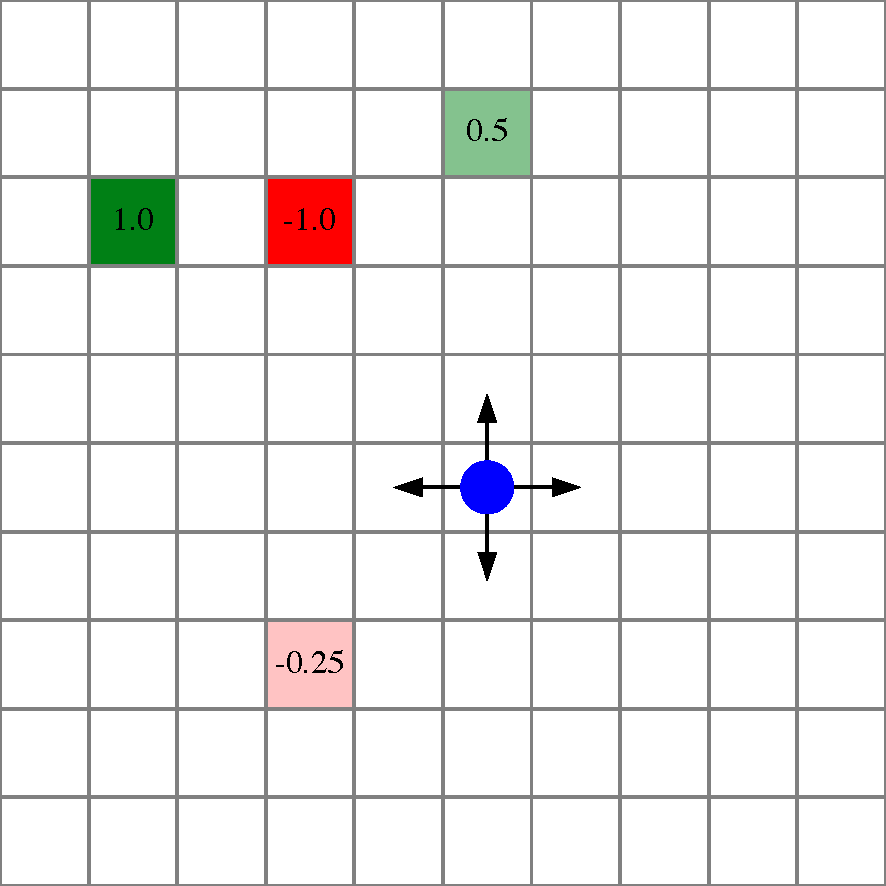
\includegraphics[width=0.5\textwidth]{figures/sample_systems/simple_gridworld.pdf}
    \caption{Simple Gridworld MDP.}
    \label{fig:simple_gridworld}
\end{figure}

% Adversarial MDP
The adversarial version of the simple gridworld is described by the failure condition, disturbance space, and disturbance model.  We define a failure as any time the agent reaches a terminal state with negative reward. The disturbances are the stochastic transitions of the agent so the disturbance space is the same as the action space of the base MDP: [\emph{up}, \emph{down}, \emph{left}, \emph{right}]. The probability of a disturbance is in state $s$ is
\begin{equation}
    p(x \mid s) = \begin{cases}
    p_{\rm success} & \text{if } x = \pi(s) \\
    (1 - p_{\rm success}) / 3 & \text{if } x \neq \pi(s) \\ 
    \end{cases}
\end{equation}
The reward function and discount factor are task and solver dependent and will be discussed in the description of the safety validation experiments. 

% Implementation details
The implementation of both the base and adversarial MDP can be done using the \texttt{SimpleGridworld} MDP distributed as part of the POMDPModelTools.jl\footnote{https://github.com/JuliaPOMDP/POMDPModelTools.jl} package. The base MDP can be implemented by defining the grid size, the value and location of the rewards, the states to terminate from, and the probability of a successful transition. The adversarial MDP can then be constructed with the same size and terminal states, but the rewards are now set to \num{1} for each failure state in the base MDP, and \num{0} for all others. The probability of transition success is set to \num{1} so that the actions of the adversarial MDP completely control the agent.



\subsection{Gridworld with Adversary}
% Base MDP
In order to increase the difficulty of the safety validation problem we introduce a new gridworld variation that includes an adversarial agent (shown in \cref{fig:gridworld_with_adversary}). Two agents move on an $N_x \times N_y$ gridworld: the ego agent (in blue) tries to reach states with high reward, while the adversary (in orange) tries to collide with the ego agent. The state of the environment is the grid location of each agent and the action space is [\emph{up}, \emph{down}, \emph{left}, \emph{right}, \emph{stay}, \emph{up-right}, \emph{up-left}, \emph{down-right}, \emph{down-left}], which control the transitions of the ego agent. For each episode the agents are initialized to a random non-terminal position. On each iteration both agents select an action and then transition to the corresponding cell with probability $p_{\rm success}$, or to another adjacent cell with probability $1-p_{\rm success}$. Some states are marked as impassible (shown in black), so if the agent would transition to an impassible state or out of bounds of the gridworld then it stays in its current state. The episode terminates when the ego agent reaches a terminal state (any state with positive reward) or the two agents overlap in the same state. The state space of this MDP is the square of the simple gridworld, but for modestly sized grids, dynamic programming is tractable for solving for the optimal ego policy. 

\begin{figure}
    \centering
    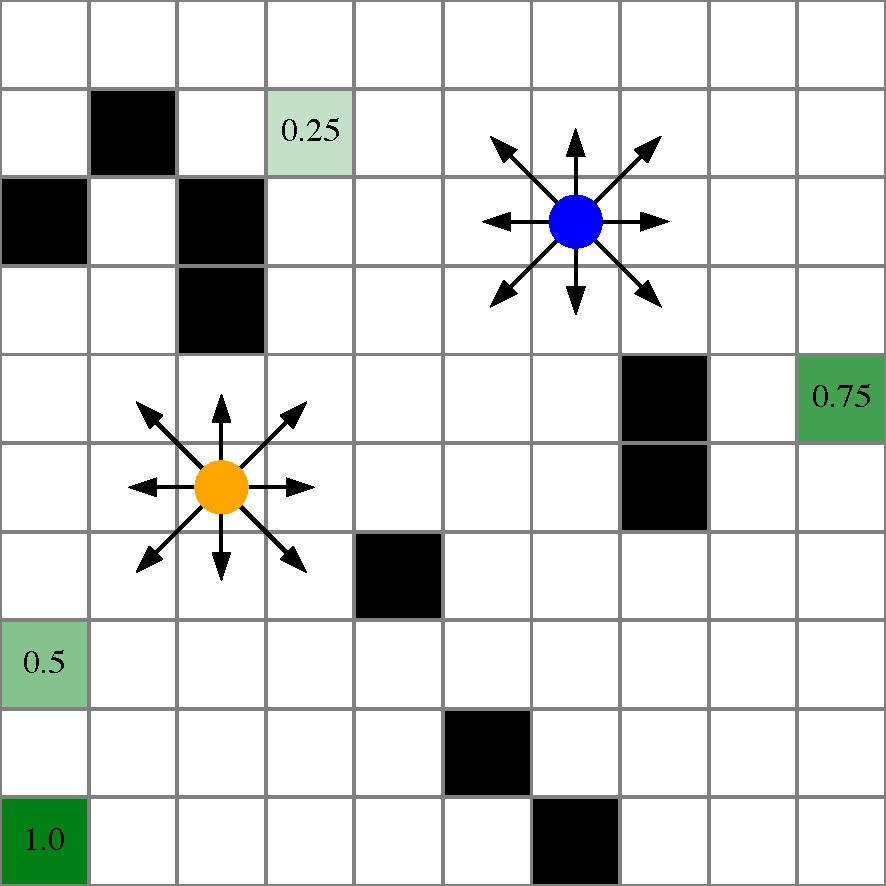
\includegraphics[width=0.5\textwidth]{figures/sample_systems/gridworld_with_adversary.pdf}
    \caption{Gridworld with Adversray MDP.}
    \label{fig:gridworld_with_adversary}
\end{figure}

For the adversarial MDP, we define a failure of the ego agent as a collision between the ego agen and the adversary. The disturbances are the actions of the adversarial agent and so the disturbance space is the same as the action space in the base MDP. The probability of each disturbance can be user specified. If we assume that the adversary moves entirely at random, then the probability of each disturbance would be $p(x \mid s) = 1 / 9$.

Both the base MDP and the adversarial MDP can be implemented using the julia package AdversarialGridworld.jl\footnote{https://github.com/sisl/AdversarialGridworld.jl}. A gridworld with an adversary is defined by specifying the grid size, the location of terminal states, the rewards, and the location of impassible states and the probability of successful transitions $p_{\rm success}$. The MDP can be switched between base mode and adversarial mode. In base mode, the actions of the MDP correspond to the actions of the ego agent and the reward function returns positive reward when the ego agent reaches a reward state and negative reward for a collision. In adversarial mode, the actions of the MDP correspond to the adversary and the reward function gives a positive reward for collisions. In both modes, the agent that is not controlled by the actions of the MDP must have a policy associated with it.

\section{Autonomous Driving}
% Why autonomous vehicles
To complement the simplicity of the gridworld MDPs, we introduce two MDPs to model autonomous driving behavior in complex environments. Autonomous driving is an especially important domain for safety validation due to the recent development and deployment of autonomous vehicles~\cite{koopman2016challenges}. Safety validation of an autonomous driving policy is challenging due to the size of the state and disturbance spaces, the duration of the diving episodes, and the rarity of failure events.

% How we model driving and adversarial driving MDPs
To model driving scenarios in simulation we build off of the julia package AutomotiveSimulator.jl\footnote{https://github.com/sisl/AutomotiveSimulator.jl} which provides methods for constructing road geometries, vehicles, pedestrians and behavior models. To facilitate the construction of adversarial MDPs for driving scenarios, we developed the package AdversarialDriving.jl\footnote{https://github.com/sisl/AdversarialDriving.jl}. Adversarial driving scenarios are constructed from a set of agents where each agent is defined by
\begin{itemize}
    \item An \emph{initialization function} that generates the initial state of the agent. The function may be deterministic or randomized, and is called each time the MDP is reset. 
    \item A \emph{behavior model} that determines the actions of the agent. For the system under test, the behavior model implements the autonomous driving policy we wish to test. For adversaries, the model implements their behavior and disturbances.
    \item A \emph{disturbance model} that is a probability distribution over disturbances which can be used to sample disturbances and compute their probability. 
\end{itemize}

% Description of the state space, action space, and  dynamics
The MDP is constructed with an agent representing the system (called the ego vehicle), a vector of agents that act as the adversaries (either other vehicles or pedestrians), a road geometry, and the simulation timestep. The state and action spaces are dynamically constructed based on the number and type of agents in the scene. We assume that vehicles stay in their lane during the simulation and can therefore specify a vehicle's state using four state variables ($r$, $v$, $\ell$, $b$) where $r$ is the position along the lane, $v$ is the speed of the vehicle in the direction of the lane, $\ell$ is an integer representing which lane the vehicle is in, and $b$ is a Boolean that indicates if the vehicle's turn signal is on. Pedestrians can move in any direction so their state is described by two position and two velocity variables ($r_x$, $r_y$, $v_x$, $v_y$). At each step, vehicles can apply an acceleration in the direction of the direction of the lane and pedestrians can apply a 2D acceleration. The position and velocity of each agent (in each direction) is updated by the kinematic relation
\begin{equation}
\begin{split}
    r_{t+\Delta t} &= r_t + v_t \Delta t + \frac{1}{2} a_t \Delta t^2 \\
    v_{t+\Delta t} &= v_t + a_t \Delta t
    \end{split}
    \label{eq:kinematics}
\end{equation}
where $\Delta t$ is the simulation timestep. Additionally, vehicles that have the opportunity to make a turn can toggle their intention to turn and whether or not their turn signal is on. The policies we use to control agents in the scene are Markov, so the simulation can be initialized into an arbitrary state.


% Description of the intelligent driving model
The driving policy that we use for vehicles is based on the intelligent driver model (IDM), a rule-based algorithm that applies longitudinal acceleration to reach a desired velocity while avoiding rear-end collisions. The IDM algorithm is shown in \cref{alg:idm}. It takes as input the current separation between the ego vehicle and the agent ahead of it $\Delta s$, the velocity of the ego $v_{\rm ego}$, and the velocity of the lead vehicle $v_{\rm lead}$. If there is no lead vehicle then $\Delta s = \infty$ and $v_{\rm lead} = {\rm NaN}$. In the presence of a leading vehicle (line \ref{line:idm_has_lead}), the IDM computes a desired following distance (line \ref{line:idm_compute_desired}) and then computes an acceleration to match the desired velocity and following distance (line \ref{line:idm_compute_acc}). If there is no leading vehicle (line \ref{line:idm_nolead}) then the acceleration is computed to gradually approach the desired driving velocity (line \ref{line:idm_compute_acc_free}). The behavior of the IDM is governed by a set of driving parameters which are shown in \cref{tab:idm_params} with their default values. 


\begin{table}
    \centering
    \caption{Default IDM parameter values.}
    \label{tab:idm_params}
    \begin{tabular}{@{}lll@{}} 
        \toprule
        \textbf{Description} & \textbf{Variable} & \textbf{Default Value} \\
        \midrule
        Speed tracking constant & $k$ & \SI{1.0}{s^{-1}} \\
        Acceleration exponent & $\delta$ & \num{4.0} \\
        Desired time headway & $T_{\rm des}$ & \SI{1.5}{s}\\
        Minimum allowed gap & $r_{\rm min}$ & \SI{5.0}{m} \\
        Desired velocity & $v_{\rm des}$ & \SI{29.0}{m/s} \\
        Maximum acceleration & $a_{\rm max}$ & \SI{3.0}{m/s^2} \\
        Comfortable deceleration & $d_{\rm comf}$ & \SI{2.0}{m/s^2} \\
        Maximum deceleration & $d_{\rm max}$ & \SI{9.0}{m/s^2} \\
        \bottomrule
    \end{tabular}
    \vskip -0.2in
\end{table}


 \begin{algorithm}
\caption{Intelligent Driver Model.}
    \label{alg:idm}
\begin{algorithmic}[1]
    \Function{IDMAcceleration}{$\Delta r$, $v_{\rm ego}$, $v_{\rm lead}$}
    \State $\Delta v \gets v_{\rm lead} - v_{\rm ego}$
    \If{$v_{\rm lead} \neq \rm{NaN}$} \label{line:idm_has_lead}
        \State $r_{\rm des} = r_{\rm min} + v_{\rm ego} \Delta T_{\rm des} - \frac{v_{\rm ego} \Delta v}{2 \sqrt{a_{\rm max} d_{\rm comf}}}$ \label{line:idm_compute_desired}
        \State $a \gets a_{\rm max} \left( 1 - \left(\frac{v_{\rm ego}}{v_{\rm des}} \right)^{\delta} - \left( \frac{r _{\rm des}}{\Delta r} \right)^2 \right)$ \label{line:idm_compute_acc}
    \Else \label{line:idm_nolead}
        \State $a \gets k \Delta v$ \label{line:idm_compute_acc_free}
    \EndIf
    \State \textbf{return} \textproc{clamp}($a$, $-d_{\rm max}$, $a_{\rm max}$) \label{line:idm_clamp_acc}
    \EndFunction
\end{algorithmic}
\end{algorithm}


% Describe the intersection algorithm
The intelligent driving model works well for traffic on a single roadway, but is not designed to handle intersections. To allow the autonomous vehicle to navigate intersections we developed a rule-based intersection navigation algorithm that uses the IDM (shown in \cref{alg:intersection_navigation}). The algorithm takes as input the ego vehicle $veh$ that is being controlled, the $scene$ that contains the other agents on the road, and the $roadway$ which describes the road geometry. We first determine the velocity and relative position of any agent in the same lane as the ego vehicle (line \ref{line:intersectionidm_leading_vehicle}). 
If there is no leading vehicle, then the velocity will be $v_{\rm lead} = {\rm NaN}$ and the relative position will be infinite. We then check if the ego vehicle has right of way in the intersection (line \ref{line:intersection_if_ROW}), and if it does, the vehicle proceeds with the IDM acceleration (line \ref{line:intersection_regular_idm_acc}). The right of way rules are 1) vehicles going straight have priority over vehicles that are turning and 2) vehicles turning right have priority over vehicles turning left. If a vehicle has a turn signal on, them it is assumed to be turning and vice versa. 

If the vehicle does not have right of way then the distance to the intersection (line \ref{line:intersection_distance2intersection} and the time it will take to cross it (line \ref{line:intersection_timetocross}) are computed and used to determine if the intersection is occupied. The intersection is considered occupied if for any other agent on the road, that agent is already in the intersection or, based on its current velocity, will be in the intersection during the planned crossing time of the ego vehicle. If the intersection is occupied and the lead vehicle has already passed the intersection then we use the stationary boundary of the intersection as the reference point for the IDM (line \ref{line:intersection_idm2int}), and otherwise we use the leading vehicle still (line \ref{line:intersection_regular_idm_acc2}).


 \begin{algorithm}
\caption{Intersection navigation algorithm.}
    \label{alg:intersection_navigation}
\begin{algorithmic}[1]
    \Function{IntersectionIDMAcceleration}{$veh$, $scene$, $roadway$}
        \State $v \gets$ \textproc{Velocity}($veh$)
        \State $v_{\rm lead}$, $\Delta s_{\rm lead} \gets$ \textproc{LeadingVehicle}($veh$, $scene$) \label{line:intersectionidm_leading_vehicle}
        \If{\textproc{HasRightOfWay}($veh$, $scene$, $roadway$)} \label{line:intersection_if_ROW}
            \State \textbf{return} \textproc{IDMAcceleration}($\Delta s_{\rm lead}$, $v$, $v_{\rm lead}$) \label{line:intersection_regular_idm_acc}
        \Else
            \State $\Delta s_{\rm int} \gets$ \textproc{DistanceToIntersection}($veh$, $roadway$) \label{line:intersection_distance2intersection}
            \State $\Delta t_{\rm cross} \gets$ \textproc{TimeToCrossIntersection}($veh$, $roadway$)  \label{line:intersection_timetocross}
            
            \If{\textproc{IntersectionOccupied}($scene$, $roadway$, $\Delta t_{\rm cross}$) and $\Delta s_{\rm int} < \Delta s_{\rm lead}$} \label{line:intersection_occupied}
                \State \textbf{return} \textproc{IDMAcceleration}($\Delta s_{\rm int}$, $v$, \num{0}) \label{line:intersection_idm2int}
            \Else
                \State \textbf{return} \textproc{IDMAcceleration}($\Delta s_{\rm lead}$, $v$, $v_{\rm lead}$) \label{line:intersection_regular_idm_acc2}
            \EndIf
        \EndIf
    \EndFunction
\end{algorithmic}
\end{algorithm}

% Assumptions used for the intersection navigation algorithm
The intersection navigation algorithm relies on several assumptions to make it functional. For sensing, it assumes that the ego vehicle can noisily observe all other agents in the scene (no occlusions), and has perfect knowledge of the road geometry (such as the location of any intersections). For the behavioral modeling of other agents, it assumes that an agent will turn on its turn signal if and only if it is turning, and that other agents drive with a constant velocity when approaching the intersection. Any violation of these assumptions could lead to a collision. The goal of this driving policy, however, is not to build an industrial autonomous driving planner, but to construct a driving policy that exhibits complex driving behavior while avoiding most collisions. Weaknesses in the algorithm provide potential failure modes that we can investigate with the safety validation algorithms developed in later chapters. 

% Low fidelity simulation
The simulation environment is lower fidelity than simulators used in industry.  For example, the motion of the agents is controlled by point-mass dynamics instead of the complex 3D dynamics of a real vehicle or pedestrian. The environment is not rendered photo-realistically, so advanced perception systems cannot be used. The driving policy does not have machine-learned components and is assumed to be Markov. Despite these differences we have designed the autonomous driving scenarios to have similar state spaces, actions spaces, number of interacting agents and rarity of failure events to those of an industrial simulator and driving policy. Due to the this matching, we believe that safety validation algorithms that work for the following scenarios will be applicable to real-world autonomous driving simulators.


\subsection{Pedestrian in Crosswalk}
% Description of the base MDP
In the pedestrian crosswalk MDP shown in \cref{fig:pedestrian_crosswalk}, an autonomous vehicle approaches a crosswalk where a pedestrian is attempting to cross. The vehicle makes noisy observations of the pedestrian's position and velocity, and uses those observations with the intersection navigation algorithm (\cref{alg:intersection_navigation}) to determine its acceleration. Since there is only a single lane for the vehicle, the state space of the vehicle can be reduced to the longitudinal position and velocity ($r_x^{\rm veh}$, $v_x^{\rm veh}$) while the state of the pedestrian is the lateral and longitudinal position and velocity ($r^{\rm ped}_x$, $r^{\rm ped}_y$, $v^{\rm ped}_x$, $v^{\rm ped}_y$). The action space of the vehicle is the range of accelerations between $[-d_{\rm max}, a_{\rm max}]$. At the start of each episode, both agents are initialized randomly with the vehicle driving in the positive $x$-direction and the pedestrian is on the right side of the vehicle. At each step, both agents determine their accelerations and their position and velocity are updated according to the kinematic relations in \cref{eq:kinematics}. The episode ends if there is a collision between the vehicle and the pedestrian or if the vehicle makes it to the end of the roadway. Since the driving policy is rule-based and does not require any learning, we have no need to explicitly specify a reward for the base MDP. 

\begin{figure}
    \centering
    \begin{tikzpicture}
         \node (fig1) at (0,0)
           {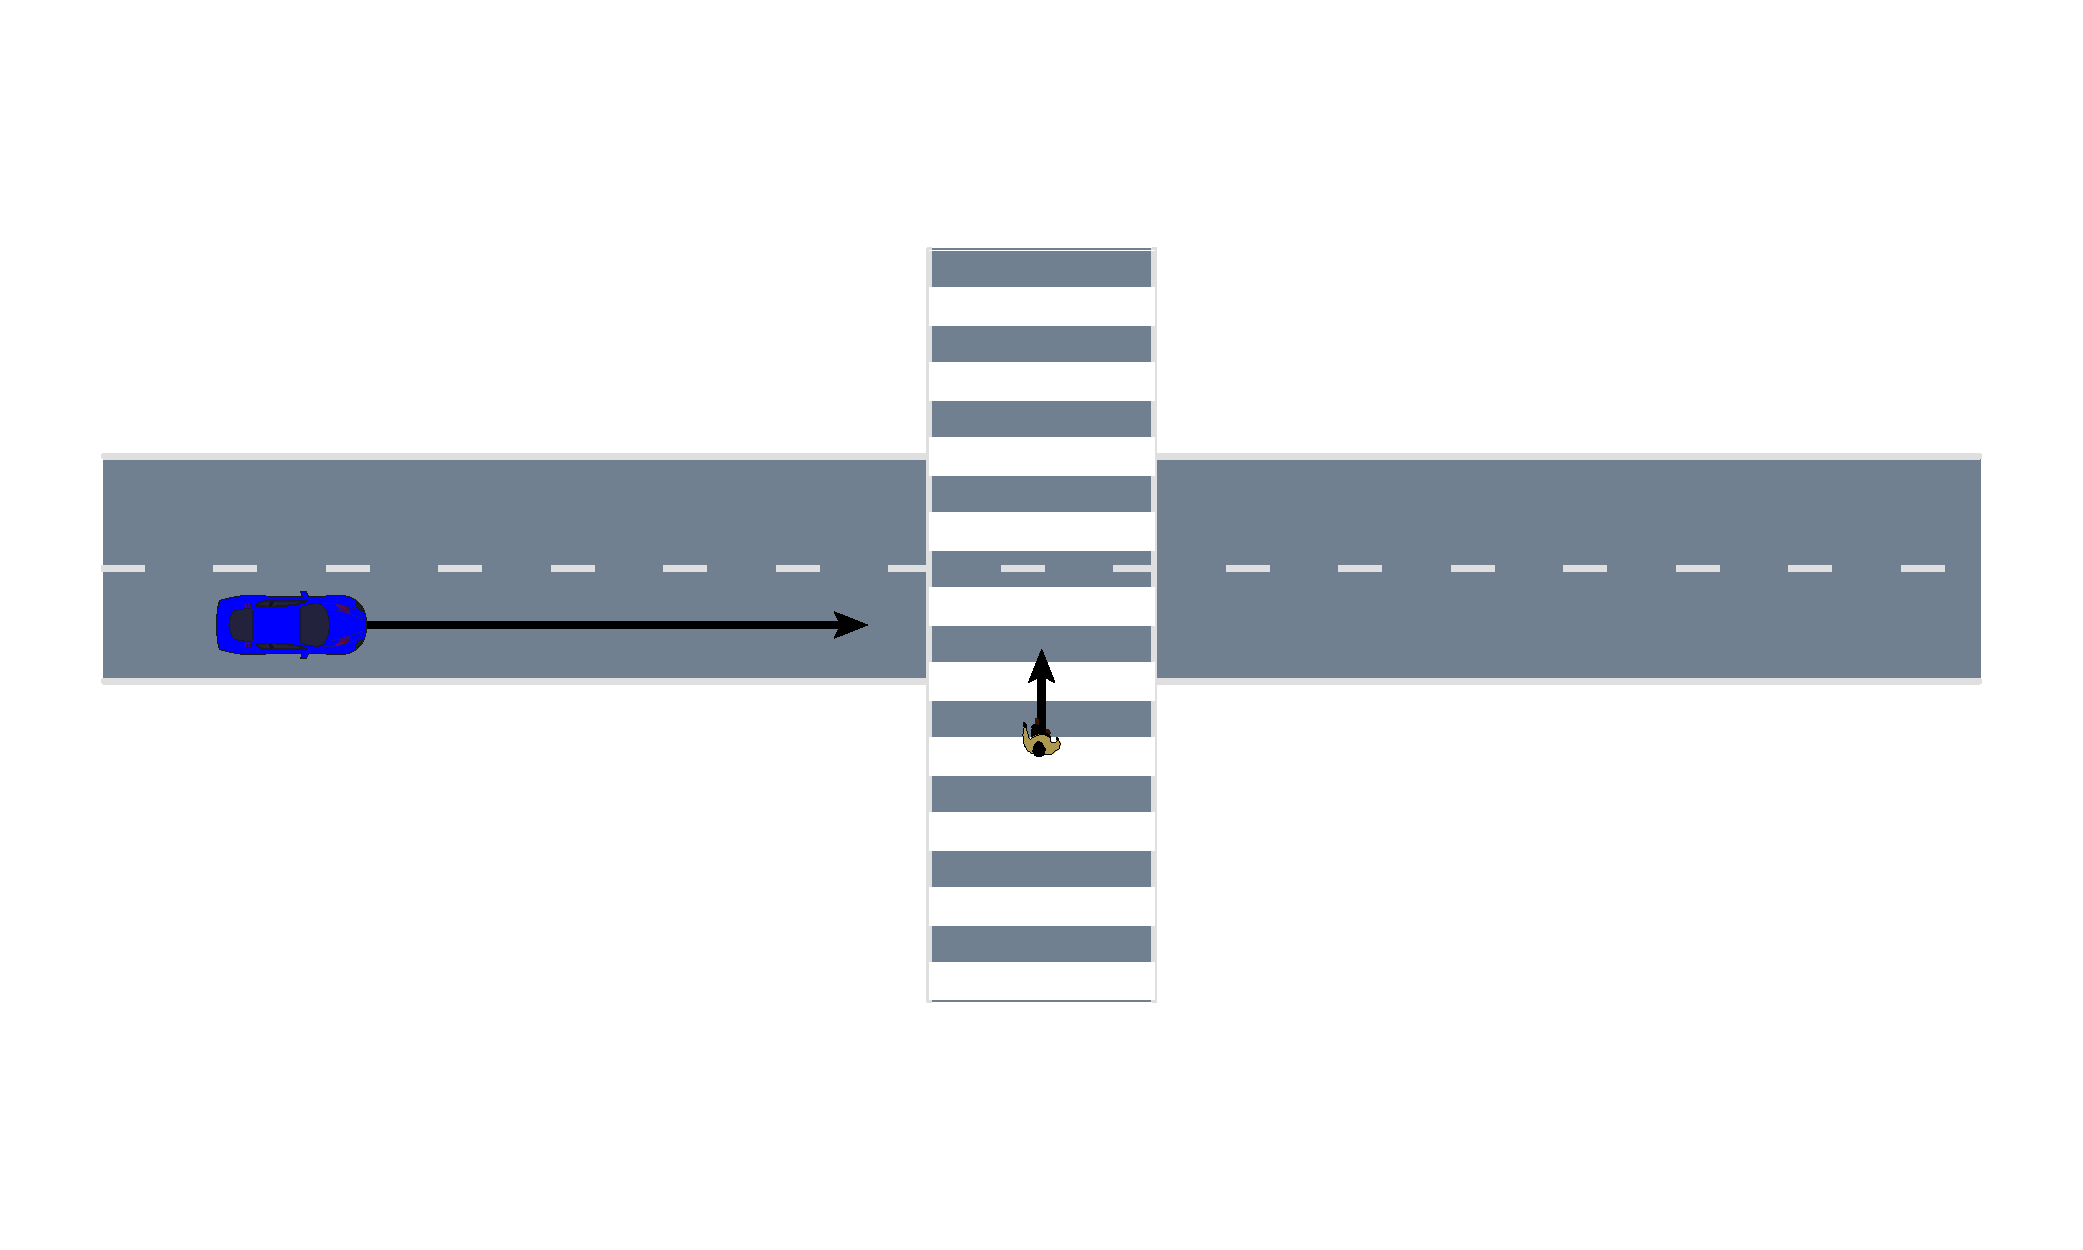
\includegraphics[trim={0 5cm 0 5cm},clip, width=\textwidth]{figures/sample_systems/pedestrian_crosswalk.pdf}};
         \draw[->] (5,-2.3)--(6,-2.3) node[right]{$x$};
         \draw[->] (5,-2.3)--(5,-1.4) node[above]{$y$};
    \end{tikzpicture}
    \caption{Crosswalk MDP where the ego vehicle approaches a crosswalk while a pedestrian tries to cross. }
    \label{fig:pedestrian_crosswalk}
\end{figure}


% Description of the adversarial MDP
Failures of this scenario are defined by any collision between the pedestrian and vehicle. The disturbances are the longitudinal and lateral accelerations of the pedestrian ($\delta a_x$ $\delta a_y$), and the longitudinal and lateral noise in the measurement of the pedestrian's position and velocity ($\delta n_x$, $\delta n_y$, $\delta n_{v_x}$, $\delta n_{v_y}$). All six disturbances are continuous but if we are using a safety validation solver that requires a discrete disturbance space, then we can discretize them. If we assume that the disturbances are independent then we can model each with a zero-mean Gaussian distribution. If we want to model correlated disturbances to better caption human-like behavior, we can model them as Gaussian processes with kernel function $\vec{k}$ and mean function $\vec{\mu}$. These options are shown in \cref{tab:adversarial_ped_disturbance_space}.


\begin{table}
    \centering
    \caption{Continuous disturbance space for adversarial pedestrian in crosswalk MDP.}
    \label{tab:adversarial_ped_disturbance_space}
    \begin{tabular}{@{}lrr@{}} 
        \toprule
        \textbf{Disturbance} & \textbf{Independent} & \textbf{Correlated} \\
        \midrule
        Longitudinal Acceleration &  $\delta a_x \sim \mathcal{N}(0, \sigma_{a_x}^2)$ &  $\vec{\delta a}_x \sim \mathcal{N}(\vec{\mu}_{a_x}(\vec{t}), \vec{k}_{a_x}(\vec{t}, \vec{t}))$ \\
        Lateral Acceleration &  $ \delta a_y \sim \mathcal{N}(0, \sigma_{a_y}^2)$ &  $\vec{\delta a}_y \sim \mathcal{N}(\vec{\mu}_{a_y}(\vec{t}), \vec{k}_{a_y}(\vec{t}, \vec{t}))$ \\
        Longitudinal Acceleration &  $\delta n_x \sim \mathcal{N}(0, \sigma_{r_x}^2)$ &  $\vec{\delta n}_x \sim \mathcal{N}(\vec{\mu}_{r_x}(\vec{t}), \vec{k}_{r_x}(\vec{t}, \vec{t}))$ \\
        Lateral Position Noise &  $\delta n_y \sim \mathcal{N}(0, \sigma_{r_y}^2)$ &  $\vec{\delta n}_y \sim \mathcal{N}(\vec{\mu}_{r_y}(\vec{t}), \vec{k}_{r_y}(\vec{t}, \vec{t}))$ \\
        Longitudinal Velocity Noise &  $\delta n_{v_x} \sim \mathcal{N}(0, \sigma_{v_x}^2)$ &  $\vec{\delta n}_{v_x} \sim \mathcal{N}(\vec{\mu}_{v_x}(\vec{t}), \vec{k}_{v_x}(\vec{t}, \vec{t}))$ \\
        Lateral Velocity Noise &  $\delta n_{v_y} \sim \mathcal{N}(0, \sigma_{v_y}^2)$ &  $\vec{\delta n}_{v_x} \sim \mathcal{N}(\vec{\mu}_{v_y}(\vec{t}), \vec{k}_{v_y}(\vec{t}, \vec{t}))$ \\
        \bottomrule
    \end{tabular}
\end{table}
 



\subsection{T-Intersection}

% Base MDP
In the T-intersection MDP (shown in \cref{fig:t_intersection}), the ego vehicle tries to make an unprotected left turn onto a two-lane through-street with other vehicles at the intersection. The state of the $i$th vehicle is ($r_i$, $v_i$, $\ell_i$, $b_i$) where $r_i$ and $v_i$ are the position and velocity along lane $\ell_i$, and $b_i$ is a Boolean indicating if the vehicle's turn signal is on. The intersection is composed of \num{6} lanes: $\ell = 1$ is the lane that goes straight from left to right, $\ell = 2$ starts as lane \num{1} but turns right, $\ell = 3$ is the lane that goes straight from right to left, $\ell = 4$ starts as lane \num{3} but turns left, $\ell = 5$ turns left onto the through street, and $\ell = 6$ turns right onto the through street. Vehicles that are on the through-street can change their turn intention by changing their lane prior to the intersection. For example, a vehicle going straight in lane \num{1} can choose to turn right by switching to lane \num{2} before the turn. Each lane has at most one other lane that a vehicle could switch to without changing its position, so changing lanes can be considered an operation that toggles \emph{turn intention}.

At the start of each episode, the agents are randomly initialized into a configuration that would lead to no collisions in the absence of disturbances. On each step, each vehicle on the road makes observations of the other agents and uses \cref{alg:intersection_navigation} to determine their acceleration to safely travel through the intersection. The episode terminates when there is a collision between any two vehicles or when the ego vehicle successfully makes the left turn and reaches the end of the roadway. 

\begin{figure}
    \centering
    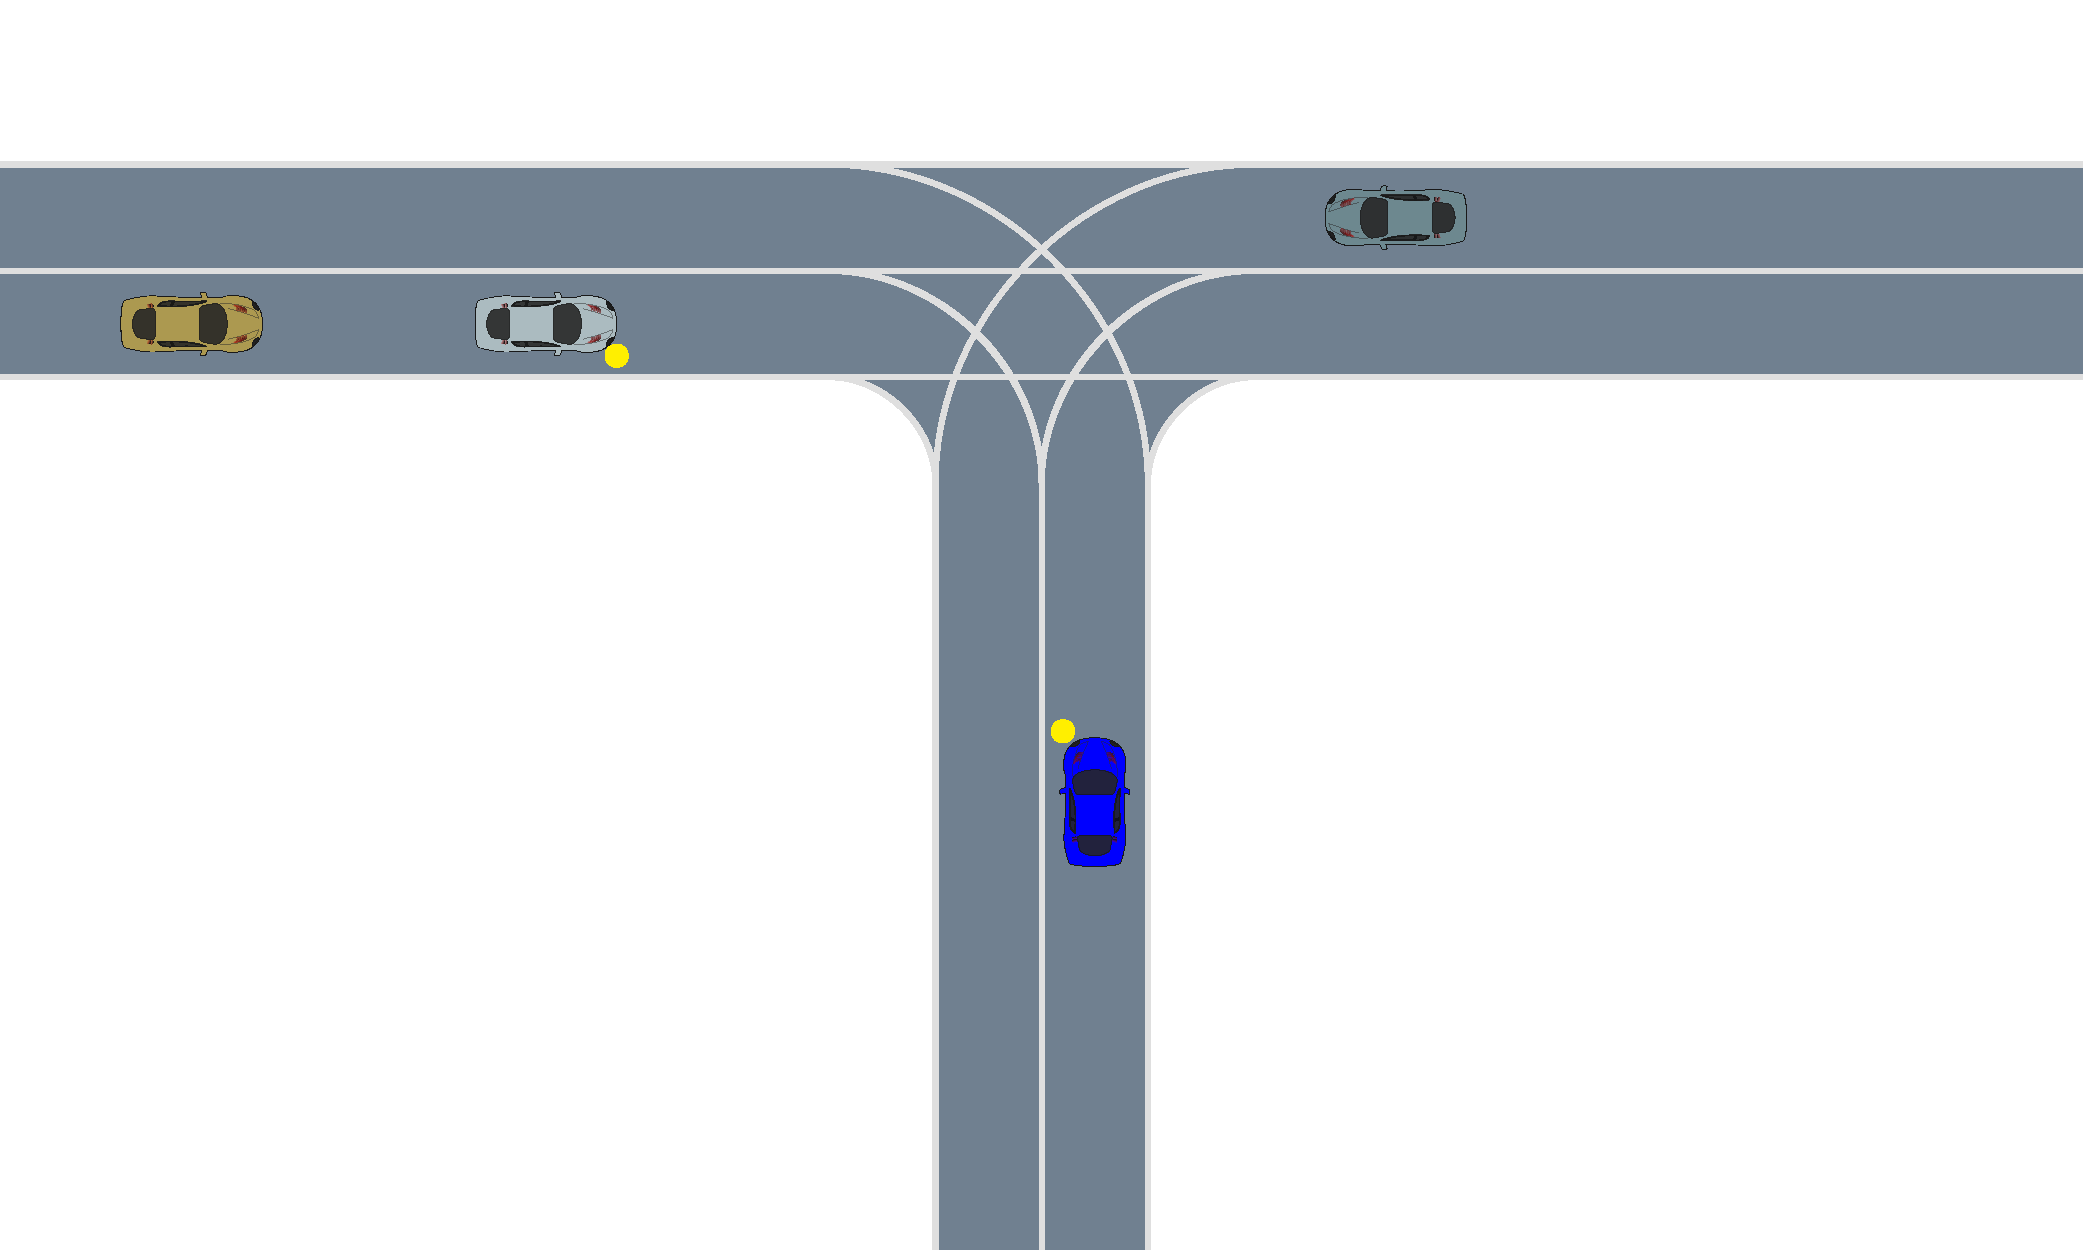
\includegraphics[trim={0 5cm 0 0},clip, width=\textwidth]{figures/sample_systems/T_intersection.pdf}
    \caption{T-Intersection MDP where the ego vehicle tries to take unprotected left turn. }
    \label{fig:t_intersection}
\end{figure}

% Adversarial MDP
In the adversarial MDP, a failure is any collision between the ego vehicle and another vehicle on the road. For each vehicle (other than the ego), the disturbances are perturbations to the vehicle's acceleration $\delta a$, toggling turn intention $\delta \ell$, or toggling the turn signal $\delta b$. If we treat the acceleration disturbance as continuous, then the disturbances can be modeled by the distributions shown in \cref{tab:Tint_continuous_disturbance_space}. If we require discrete disturbances then we can choose \num{7} representative disturbances and their associate probabilities as shown in \cref{tab:Tint_discrete_disturbance_space}.

\begin{table}
    \centering
    \caption{Continuous disturbance space for adversarial vehicles in T-intersection MDP.}
    \label{tab:Tint_continuous_disturbance_space}
    \begin{tabular}{@{}lrr@{}} 
        \toprule
        \textbf{Disturbance} & \textbf{Distribution} \\
        \midrule
        Acceleration &  $\delta a \sim \mathcal{N}(0, \sigma_a^2)$ \\
        Toggle turn intent & $\delta \ell \sim {\rm Bern}(\rho_I)$ \\
        Toggle turn signal & $\delta b \sim {\rm Bern}(\rho_S)$\\
        \bottomrule
    \end{tabular}
\end{table}

\begin{table}
    \centering
    \caption{Discrete disturbance space for adversarial vehicles in T-intersection MDP.}
    \label{tab:Tint_discrete_disturbance_space}
    \begin{tabular}{@{}lrr@{}} 
        \toprule
        \textbf{Disturbance} & \textbf{Acceleration} & \textbf{MC Probability} \\
        \midrule
        No disturbance &  \SI{0}{m/s^2} & \num{0.976}\\
        Medium slowdown & \SI{-1.5}{m/s^2} & \num{1e-2}\\
        Major slowdown & \SI{-3}{m/s^2} & \num{1e-3}\\
        Medium speedup & \SI{1.5}{m/s^2} & \num{1e-2}\\
        Major speedup & \SI{3}{m/s^2} & \num{1e-3}\\
        Toggle blinker & N/A & \num{1e-3 }\\
        Toggle turn intent & N/A & \num{1e-3} \\
        \bottomrule
    \end{tabular}
    \vskip -0.2in
\end{table}

\section{Discussion}

In this chapter we introduced the idea of an adversarial MDP to model the safety validation of an autonomous policy for a base MDP. Both MDPs share the same state space and transition model, but the actions of the base MDP are the actions of the system while the actions of the adversarial MDP are the disturbances. The adversarial MDP is a flexible model that can be used in conjunction with safety validation algorithms based on optimization, path-planning, reinforcement learning, and importance sampling.

We then introduced four safety validation problems that are used to test the safety validation algorithms developed in the remainder of this thesis. The first scenario involves the safety validation of a simple gridworld policy where the disturbances are the stochastic transitions of the agent. The second scenario is also a gridworld problem, but with another adversarial agent that causes collisions. The next two systems model autonomous driving scenarios. In the first, the ego vehicle approaches a crosswalk with a crossing pedestrian and must avoid the pedestrian under disturbances to the pedestrian motion and sensor noise. The second driving scenario is a T-intersection where the ego vehicle makes an unprotected left turn onto a through-street with other drivers on the road. The disturbances are the behavior of other vehicles on the road and include perturbations to the acceleration, toggling of turn intention and toggling the turn signal.

The following chapter begins the development of safety validation algorithms. We introduce a technique for interpretable safety validation and demonstrate it with the autonomous driving scenarios. 